\documentclass{article}[11pt]

\usepackage{amsmath}
\usepackage{amssymb}
\usepackage{nicefrac}

\usepackage{pdflscape}

\usepackage{upgreek}

\usepackage{bashful}

% No intendation
\setlength\parindent{0pt}

\usepackage{hyperref}

\usepackage{siunitx}
\sisetup{
  per-mode=fraction,
  fraction-function=\tfrac
}

\usepackage{listings}
  \lstset{
    basicstyle=\ttfamily,
    escapeinside=||,
    xleftmargin=1cm
  }

\usepackage{float}

\usepackage{longtable}

\usepackage{multirow}

\usepackage{tikz}
  \usetikzlibrary{patterns}
  \usetikzlibrary{arrows.meta}
  \usetikzlibrary{shapes.misc}
  \usetikzlibrary{calc}

\usepackage{pgfplots}

\usepackage{cleveref}
\crefmultiformat{equation}{(#2#1#3)}{ and~(#2#1#3)}{, (#2#1#3)}{ and~(#2#1#3)}


\usepackage{acronym}
\usepackage[acronym,nonumberlist]{glossaries}
\glsdisablehyper
\makeglossaries
\newacronym{spice}{SPICE}{Simulation Program with Integrated Circuit Emphasis}
\newacronym{lef}{LEF}{Library Exchange Format}
\newacronym{dft}{DFT}{Discrete Fourier Transform}
\newacronym{dtft}{DTFT}{Discrete-Time Fourier Transform}
\newacronym{fft}{FFT}{Fast Fourier Transform}
\newacronym{mosfet}{MOSFET}{Metal–Oxide–Semiconductor Field-Effect Transistor}
\newacronym{clm}{CLM}{Channel Length Modulation}
\newacronym{de}{DE}{differential equation}
\newacronym{soi}{SOI}{silicon-on-insulator}
\newacronym{ldo}{LDO}{low-dropout regulator}
\newacronym{ota}{OTA}{operational-transconductance amplifier}
\newacronym{ofa}{OFA}{operational-floating amplifier}

% literature
\usepackage[ backend=biber
           , isbn=true
           , sorting=none
           , style=ieee
           ]{biblatex}
\addbibresource{./../../literature.bib}

% definitions
\def \whatis       {Notes}
\def \title        {Fuubar}

\def \author       {Matthias Schweikardt}

\def \authorMail   {mschweikardt@posteo.de}

\def \authorGithub {mschweikardt}

\def \license      {CC BY-SA 4.0}
\def \licenseUrl   {https://creativecommons.org/licenses/by-sa/4.0/}

\def \date         {nodate}

\def \pdfurl       {https://mschweikardt.github.io/ee-notes/%
\bash[stdout]
IFS=/ 
var=($PWD)
echo ${var[-1]}
\END%
.pdf
}
\def \srcurl       {srcurl}


% Customize footer and header of document
\usepackage{fancyhdr}

% Access last page number
\usepackage{lastpage}

% Access last page number
\usepackage[thinc]{esdiff}

% Physics
\usepackage{physics}

% Comment environment
\usepackage{comment}

% Subcaptions
\usepackage{subcaption}

% Thicker lines in tables
\usepackage{booktabs}

% Indentation in footnote
\makeatletter
\renewcommand\@makefntext[1]{\leftskip=2em\hskip-0.5em\@makefnmark#1}
\makeatother         

% qty with the siunitx definition
\AtBeginDocument{\RenewCommandCopy\qty\SI}

% TikZ compatibility
\pgfplotsset{compat=1.18}


\makeatletter
\pgfmathdeclarefunction{myatan2}{2}{%
\begingroup%
  \pgfmathfloattofixed{#1}\edef\tempa{\pgfmathresult}%
  \pgfmathfloattofixed{#2}%
  \pgfkeys{pgf/fpu=false}%
  \pgfmathparse{atan2(\tempa,\pgfmathresult)}\pgfkeys{/pgf/fpu}%
  \pgfmathfloatparsenumber{\pgfmathresult}%
  \pgfmath@smuggleone\pgfmathresult%
\endgroup
}
\makeatother

\usepackage{tabularx}
\usepackage{amsmath}
\usepackage{amssymb}
\usepackage{nicefrac}

\usepackage{pdflscape}

\usepackage{upgreek}

\usepackage{bashful}

% No intendation
\setlength\parindent{0pt}

\usepackage{hyperref}

\usepackage{siunitx}
\sisetup{
  per-mode=fraction,
  fraction-function=\tfrac
}

\usepackage{listings}
  \lstset{
    basicstyle=\ttfamily,
    escapeinside=||,
    xleftmargin=1cm
  }

\usepackage{float}

\usepackage{longtable}

\usepackage{multirow}

\usepackage{tikz}
  \usetikzlibrary{patterns}
  \usetikzlibrary{arrows.meta}
  \usetikzlibrary{shapes.misc}
  \usetikzlibrary{calc}

\usepackage{pgfplots}

\usepackage{cleveref}
\crefmultiformat{equation}{(#2#1#3)}{ and~(#2#1#3)}{, (#2#1#3)}{ and~(#2#1#3)}


\usepackage{acronym}
\usepackage[acronym,nonumberlist]{glossaries}
\glsdisablehyper
\makeglossaries
\newacronym{spice}{SPICE}{Simulation Program with Integrated Circuit Emphasis}
\newacronym{lef}{LEF}{Library Exchange Format}
\newacronym{dft}{DFT}{Discrete Fourier Transform}
\newacronym{dtft}{DTFT}{Discrete-Time Fourier Transform}
\newacronym{fft}{FFT}{Fast Fourier Transform}
\newacronym{mosfet}{MOSFET}{Metal–Oxide–Semiconductor Field-Effect Transistor}
\newacronym{clm}{CLM}{Channel Length Modulation}
\newacronym{de}{DE}{differential equation}
\newacronym{soi}{SOI}{silicon-on-insulator}
\newacronym{ldo}{LDO}{low-dropout regulator}
\newacronym{ota}{OTA}{operational-transconductance amplifier}
\newacronym{ofa}{OFA}{operational-floating amplifier}

% literature
\usepackage[ backend=biber
           , isbn=true
           , sorting=none
           , style=ieee
           ]{biblatex}
\addbibresource{./../../literature.bib}

% definitions
\def \whatis       {Notes}
\def \title        {Fuubar}

\def \author       {Matthias Schweikardt}

\def \authorMail   {mschweikardt@posteo.de}

\def \authorGithub {mschweikardt}

\def \license      {CC BY-SA 4.0}
\def \licenseUrl   {https://creativecommons.org/licenses/by-sa/4.0/}

\def \date         {nodate}

\def \pdfurl       {https://mschweikardt.github.io/ee-notes/%
\bash[stdout]
IFS=/ 
var=($PWD)
echo ${var[-1]}
\END%
.pdf
}
\def \srcurl       {srcurl}


% Customize footer and header of document
\usepackage{fancyhdr}

% Access last page number
\usepackage{lastpage}

% Access last page number
\usepackage[thinc]{esdiff}

% Physics
\usepackage{physics}

% Comment environment
\usepackage{comment}

% Subcaptions
\usepackage{subcaption}

% Thicker lines in tables
\usepackage{booktabs}

% Indentation in footnote
\makeatletter
\renewcommand\@makefntext[1]{\leftskip=2em\hskip-0.5em\@makefnmark#1}
\makeatother         

% qty with the siunitx definition
\AtBeginDocument{\RenewCommandCopy\qty\SI}

% TikZ compatibility
\pgfplotsset{compat=1.18}


\makeatletter
\pgfmathdeclarefunction{myatan2}{2}{%
\begingroup%
  \pgfmathfloattofixed{#1}\edef\tempa{\pgfmathresult}%
  \pgfmathfloattofixed{#2}%
  \pgfkeys{pgf/fpu=false}%
  \pgfmathparse{atan2(\tempa,\pgfmathresult)}\pgfkeys{/pgf/fpu}%
  \pgfmathfloatparsenumber{\pgfmathresult}%
  \pgfmath@smuggleone\pgfmathresult%
\endgroup
}
\makeatother

\usepackage{tabularx}

\input{./../../tikzlib/figs/feedback-system-a.tex}

\def \title  {Stability of Feedback Systems}
\def \date   {June 1, 2025}

\def \pdfurl {https://mschweikardt.github.io/ee-notes/feedback-stability.pdf}
\def \srcurl {https://github.com/mschweikardt/ee-notes/tree/main/notes/feedback-stability}

\usepackage[scale=5]{draftwatermark}

\usetikzlibrary{pgfplots.groupplots}

\begin{document}

\notetitle

An idealized feedback configuration is shown in Fig. \ref{fig:fs},
with the input signal is $\underline{X}(s)$ and the output signal
$\underline{Y}(s)$.
It consists of the main building block
\begin{equation}
\underline{A}(s) = \frac{\underline{Y}(s)}{\underline{Z}(s)}
\end{equation}
and the feedback network
\begin{equation}
\underline{\beta}(s) = \frac{\underline{V}(s)}{\underline{Y}(s)}.
\end{equation}
The main building block is in most cases an amplifier or an LDO 
and the feedback network is passive.
\begin{figure}[H]
  \centering
  \begin{tikzpicture}
    \FeedbackSystemA 
  \end{tikzpicture}
  \caption{Feedback system}
  \label{fig:fs}
\end{figure}

The \textit{loop gain} of the system is 
\begin{equation}
\underline{L}(s) = \frac{\underline{V}(s)}{\underline{Z}(s)} 
                 = \underline{A}(s) \cdot \underline{\beta}(s).
\end{equation}

The \textit{closed-loop gain} is
\begin{equation}\label{eq:fs}
\underline{T}(s) = \frac{\underline{Y}(s)}{\underline{X}(s)} 
                 = \frac{\underline{A}(s)}{1+\underline{L}(s)}
                 = \frac{\underline{A}(s)}{1+\underline{A}(s) \cdot \underline{\beta}(s)}.
\end{equation}

$\underline{T}(s)$ is stable only if its denominator is not zero, i.e. 
\begin{equation}
\underline{L}(s) = \underline{A}(s) \cdot \underline{\beta}(s) \neq -1.
\end{equation}

In real electronic systems, the feedback causes loading at the input and output 
of the amplifier.
As a consequence, the model shown above cannot be applied%
\footnote{The input impedance of the amplifier is in a lot of cases very high
and the output impedance very low, so therefore this model can be applied.}.

\medskip

All utilized variables in this document are summarized in 
Tab. \ref{tab:variables}.

\begin{table}[H]
\centering
\caption{Variables}
\begin{tabular}{cl}
\toprule
\textbf{Variable}       & \textbf{Description}            \\ \midrule
$\underline{X}(s)$      & Input signal                    \\ 
$\underline{Y}(s)$      & Output signal                   \\
$\underline{A}(s)$      & (open loop) transfer function   \\
$\underline{\beta}(s)$  & Feedback transfer function      \\
$\underline{L}(s)$      & Loop gain                       \\
$\underline{T}(s)$      & (closed loop) transfer function \\
$\underline{Z}(s)$      & Input signal of amplifier       \\
$\underline{V}(s)$      & Output signal of feedback       \\
$f_{\mathrm{3dB}}$      & Bandwidth                       \\
$A_{\mathrm{0}}$        & DC gain                         \\
$\mathrm{GBP}$          & Gain-Bandwidth product          \\
$\mathrm{UGBW}$         & Unity-Gain bandwidth            \\
$\mathrm{PM}$           & Phase margin                    \\
$\mathrm{GM}$           & Gain margin                     \\ \toprule
\end{tabular}
\label{tab:variables}
\end{table}

The loop gain $\underline{L}(s)$ of an exemplary system is shown in 
Fig. \ref{fig:ls}.
The magnitude is shown at the top and and phase at the bottom.

\begin{figure}[H]
  \centering
  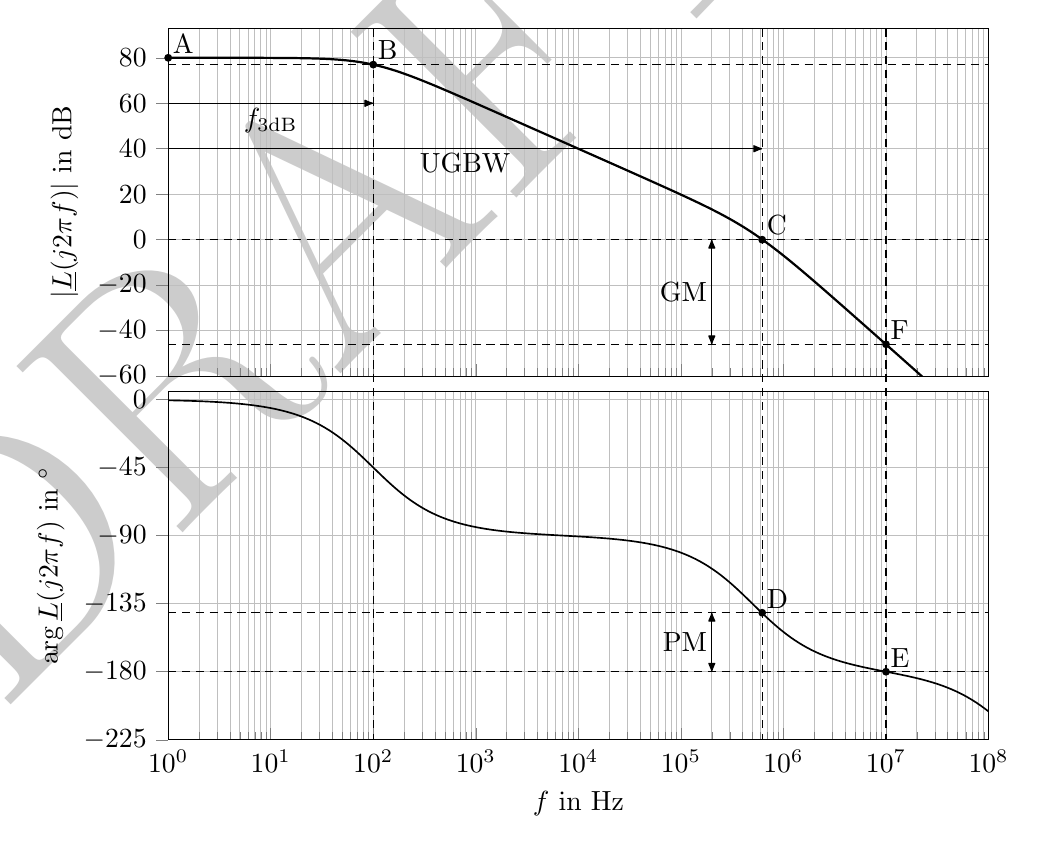
\begin{tikzpicture}
  \begin{groupplot}[
    group style={ group name=my plots
                , group size=1 by 2
                , xlabels at=edge bottom
                , xticklabels at=edge bottom
                , vertical sep=2mm
                }
      , xmode=log
      , width=12cm
      , height=6cm
      , xlabel=$f$ in \si{\hertz}
      , xmin=1
      , xmax=1e8
      , ymin=0
      , ymax=29
      , tickpos=left
      , ytick align=outside
      , grid=both
      , grid style={line width=0.3pt}
      , domain=1:1e8
      , samples=200
      ]

  \nextgroupplot[ ymin=-60
                , ymax=93
                , ytick={-80,-60,...,80}
                , ylabel= $\left|\underline{L}(j 2 \pi f)\right|$ in \si{\decibel}
                ]

    \addplot[thick] 
      ({\x},{80-10*log10(1+(\x/1e2)^2)
               -10*log10(1+(\x/5e5)^2)
               -10*log10(1+(\x/2e8)^2)});

    \coordinate (f3dbtop) at (axis cs:1e2,\pgfkeysvalueof{/pgfplots/ymax});
    \draw [densely dashed] (axis cs:1e0,0) -- (axis cs:1e8,0);
    \draw [densely dashed] (axis cs:1e0,77) -- (axis cs:1e8,77);
    \draw [densely dashed] (axis cs:1e0,-46) -- (axis cs:1e8,-46);

    \coordinate (ugbwtop) at (axis cs:6.2e5,\pgfkeysvalueof{/pgfplots/ymax});

    \coordinate (coftop) at (axis cs:1e7,\pgfkeysvalueof{/pgfplots/ymax});

    \addplot[only marks,mark=*,mark options = {scale=0.6}] coordinates{
      (1,  80)  
    };

    \node[anchor=south west, inner sep=1.5pt] at (axis cs: 1,80) {A};  

    \addplot[only marks,mark=*,mark options = {scale=0.6}] coordinates{
      (1e2,  77)  
    };

    \node[anchor=south west, inner sep=1.5pt] at (axis cs: 1e2,77) {B};  

    \addplot[only marks,mark=*,mark options = {scale=0.6}] coordinates{
      (6.2e5,  0)  
    };

    \node[anchor=south west, inner sep=1.5pt] 
      () at (axis cs: 6.2e5,  0) {C};  

    \addplot[only marks,mark=*,mark options = {scale=0.6}] coordinates{
      (1e7, -46)  
    };

    \node[anchor=south west, inner sep=1.5pt] at (axis cs: 1e7,  -46) {F};  

    \draw[ {Latex[round,scale=0.8]}-{Latex[round,scale=0.8]}]
      (axis cs: 2e5,-46) -- (axis cs: 2e5,0) 
      node[midway, left, inner sep=1.5pt] () {GM};

    \draw[-{Latex[round,scale=0.8]}]
      (axis cs: 1,60) -- (axis cs: 1e2,60) 
      node[midway, below, inner sep=1.5pt] () {$f_{\mathrm{3dB}}$};

    \draw[-{Latex[round,scale=0.8]}]
      (axis cs: 1,40) -- (axis cs: 6.2e5,40) 
      node[midway, below, inner sep=1.5pt] () {UGBW};

  \nextgroupplot[ ymin=-225
                , ymax=5
                , ylabel= $\arg\underline{L}(j 2 \pi f)$ in \si{\degree}
                , ytick={0,-45,-90,-135,-180,-225}
                ]

    \addplot[semithick]({\x},{-atan(x/1e2)-atan(x/5e5)-atan(x/2e8)}); 

    \coordinate (f3dbbot) at (axis cs:1e2,\pgfkeysvalueof{/pgfplots/ymin});

    \draw [densely dashed] (axis cs:1e0,-180) -- (axis cs:1e8,-180);

    \coordinate (ugbwbot) at (axis cs:6.2e5,\pgfkeysvalueof{/pgfplots/ymin});
    \coordinate (cofbot) at (axis cs:1e7,\pgfkeysvalueof{/pgfplots/ymin});

    \draw [densely dashed] (axis cs:1e0,-141) -- (axis cs:1e8,-141);

    \addplot[only marks,mark=*,mark options = {scale=0.6}] coordinates{
      (6.2e5,-141)  
    };

    \addplot[only marks,mark=*,mark options = {scale=0.6}] coordinates{
      (1e7,-180)  
    };

    \node[anchor=south west, inner sep=1.5pt] 
      () at (axis cs: 6.2e5,  -141) {D};  

    \node[anchor=south west, inner sep=1.5pt] 
      () at (axis cs: 1e7,  -180) {E};  

    \draw[ {Latex[round,scale=0.8]}-{Latex[round,scale=0.8]}]
      (axis cs: 2e5,-180) -- (axis cs: 2e5,-141) 
      node[midway, left, inner sep=1.5pt] () {PM};
  \end{groupplot}

  \draw [densely dashed] (f3dbtop) -- (f3dbbot);
  \draw [densely dashed] (ugbwtop) -- (ugbwbot);
  \draw [densely dashed] (coftop) -- (cofbot);
  \end{tikzpicture}
  \caption{Loop gain $\underline{L}(j 2 \pi f)$}
  \label{fig:ls}
\end{figure}


In this illustration, the phase is \SI{0}{\degree} for $f \rightarrow 0$.
In other literature, the phase is set to \SI{180}{\degree} for 
$f \rightarrow 0$%
\footnote{$\underline{L}(s) = -\underline{A}(s) \cdot \underline{\beta}(s)$}
.
Several points ($\mathrm{A}$ - $\mathrm{F}$) are annotated in the plot, each 
point has a $x$ value (corresponding to a frequency) and a $y$ value 
(corresponding either to the magnitude in dB or phase in \si{\degree}.

\medskip

By evaluating the magnitude at $f \rightarrow 0$ (point $\mathrm{A}$), the
DC gain (corresponding to $y_{\mathrm{A}}$) is extracted.
We refer to the DC gain as $A_0$ (80 dB in this example).
Next, the \SI{3}{\decibel} bandwidth $f_{\mathrm{3dB}}$ 
(a.k.a. cutoff frequency, corner frequency, or break frequency) of the
plot is evaluated. 
Therefore, we set
$$
y_{\mathrm{B}} = y_{\mathrm{A}} - 3 \mathrm{dB}
$$
and extract the matching $x_{\mathrm{B}} = f_{\mathrm{3dB}}$ 
(\SI{100}{\hertz} in this example%
\footnote{In most cases, the phase is \SI{-45}{\degree} at
$f_{\mathrm{3dB}}$.}
).
Based on that, the \textit{gain-bandwidth product}
\begin{equation}
\mathrm{GBP} = A_0 \cdot f_{\mathrm{3dB}}
\end{equation}
is calculated%
\footnote{a.k.a. $\mathrm{GBW}$, $\mathrm{GB}$}. 
You have to convert the DC gain $A_0$ from decibel in the linear domain 
beforehand (\SI{80}{\decibel} = \qty{10000}).
The $\mathrm{GBP}$ is \SI{1}{\giga\hertz} in the example shown above.
The crossover of the magnitude with \SI{0}{\decibel} 
(unity-gain, i.e. gain of one) results in the point $C$.
The x coordinate $x_{\mathrm{C}}$ of this point is the 
\textit{unity-gain bandwidth}
$\mathrm{UGBW}$%
\footnote{a.k.a. UGB, UGF}
(\SI{620}{\mega\hertz} in this example%
\footnote{It is important to notice that $\mathrm{GBP}$ is not necessarily
equal to the $\mathrm{UGBW}$.}
).
Both, $\mathrm{GBP}$ and $\mathrm{UGBW}$ are a measure for the "speed" of
the system.

\medskip

Next, we obtain the point $\mathrm{D}$ in the phase plot by setting 
$x_{\mathrm{D}} = x_{\mathrm{C}}$, i.e. evaluate the phase at the 
$\mathrm{UGBW}$.
With this point, the \textit{phase margin}

$$
\mathrm{PM} = 180° + y_{\mathrm{D}}
$$
is calculated (\SI{39}{\degree} in this example).
The phase margin is a measure for the stability of the system.

The crossover of the phase with \SI{-180}{\degree} results in the 
point $\mathrm{E}$.
By evaluating the magnitude at the same x coordinate, the point 
$\mathrm{F}$ is obtained ($x_{\mathrm{F}} = x_{\mathrm{E}}$).
With this point, the \textit{gain margin}
$$
\mathrm{GM} = - y_{\mathrm{F}}.
$$
is calculated (\SI{46}{\decibel} in this example).

\printbibliography

\end{document}